\section{Filter}\label{sec:filter_design}

The aim of this chapter is to analyse the requirements from \ref{sec:opt_result} and choose an implementation method. From the beamforming optimization it was concluded in \autoref{sec:genetic_con}, that there shall be a cost filter and a beam forming filter. This chapter starts with analysing the cost filter and design a filter solution, then the beamforming filter will be analysed and a solution will be designed.


\section{The Cost Filter}
The design of the cost filter will be done only with respect to the gain of the transfer function and without any requirements on the phase intro. The reason for neglecting the phase is, that the filter is applied to all signals in the array and therefore will not affect the beamforming. \\
The shape of the graph in \autoref{fig:opt_res_a} can be associated with a band stop filter with an additional gain increase and therefore the cost filter will be designed as a band pass filter in feedback loop. To design the cost filter, the \SI{3}{\decibel} bandwidth, the quality factor $Q$ and the gain of the filter have to be determined. To determine all required filter data, the data have to be extrapolated with an estimated function. The estimated function defined by polynomial regression with the MATLAB command \texttt{polyfit()} and with a third order regression. The third order polynomial estimates the desired transfer function of the filter. The estimation will be done from \SI{20}{\hertz} to \SI{430}{\hertz}. The \SI{430}{\hertz} choice is made such that the estimation covers at least the \SI{-3}{\decibel} bandwidth. The following \autoref{fig:band_stop_filter} shows the estimated function compared and the original data points.

\begin{figure}[H]
	\centering
	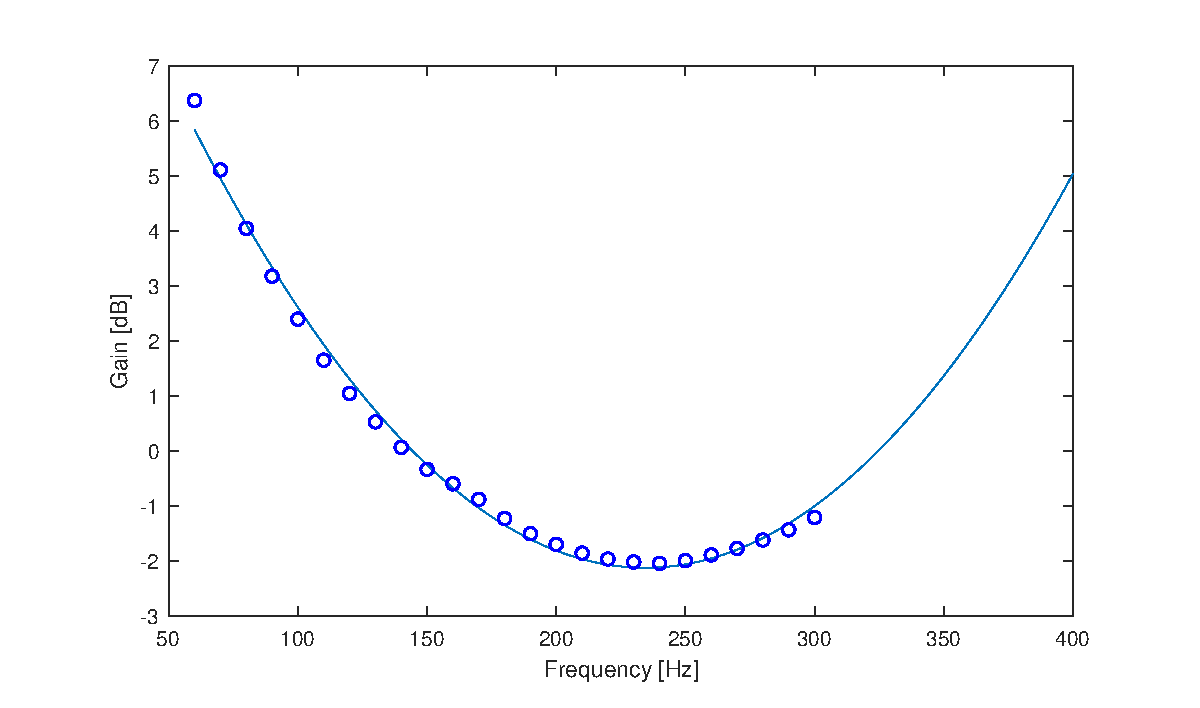
\includegraphics[width=1\textwidth]{band_stop_filter.eps}
	\caption{Estimated function for the cost filter (blue solid line) and given data points (dots).}
		\label{fig:band_stop_filter}
\end{figure}

\autoref{fig:band_stop_filter} shows, that the shape of the estimated cost transfer function can be realized with a band stop filter and a gain greater than \SI{0}{\decibel}. To achieve such filter characteristics, a design process similar to that of a parametric equalizer with a gain will be pursued. \\

\subsection{Parametric equalizer as cost filter}

To end out with a bandstop filter, first a bandpass filter is designed and then it is used in a feedback circuit. The following \autoref{fig:bandstop_filter_blockdiagram_gain} shows a block diagram of a parametric bandstop filter with input gain. 

\begin{figure}[H]
	\centering
\begin{picture}(0,0)%
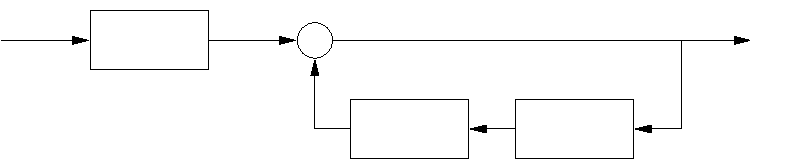
\includegraphics{bandstop_filter_blockdiagram_gain.pdf}%
\end{picture}%
\setlength{\unitlength}{4144sp}%
%
\begingroup\makeatletter\ifx\SetFigFont\undefined%
\gdef\SetFigFont#1#2#3#4#5{%
  \reset@font\fontsize{#1}{#2pt}%
  \fontfamily{#3}\fontseries{#4}\fontshape{#5}%
  \selectfont}%
\fi\endgroup%
\begin{picture}(6029,1218)(661,-973)
\put(1486,-106){In_Gain}%
\put(3196,-376){-}%
\put(3540,-781){Gain $G'$}%
\put(4681,-781){Bandpass}%
\put(2791,-286){+}%
\put(6076, 74){Output}%
\put(676, 74){Input}%
\end{picture}%
	\caption{Block diagram of a bandstop filter}
		\label{fig:bandstop_filter_blockdiagram_gain}
\end{figure}

In order to design the bandpass filter, the desired shape of the bandstop filter is mirrored and set up in a way, that the value at the center frequency is exactly \SI{0}{\decibel}.
%Designing the bandpass filter part of the bandstop filter, the bandpass filter part is changed such that the center frequency is at \SI{0}{\decibel} and the shape is a bandpass filter, not a bandstop filter. 
To convert the estimated function to a band pass, the parameters of the estimated function are inverted and attenuated by \SI{2.1}{\decibel} in order to get the extremum to \SI{0}{\decibel}. The following \autoref{fig:band_pass_filter} shows the bandpass filter characteristic, that results from this.

\begin{figure}[H]
	\centering
	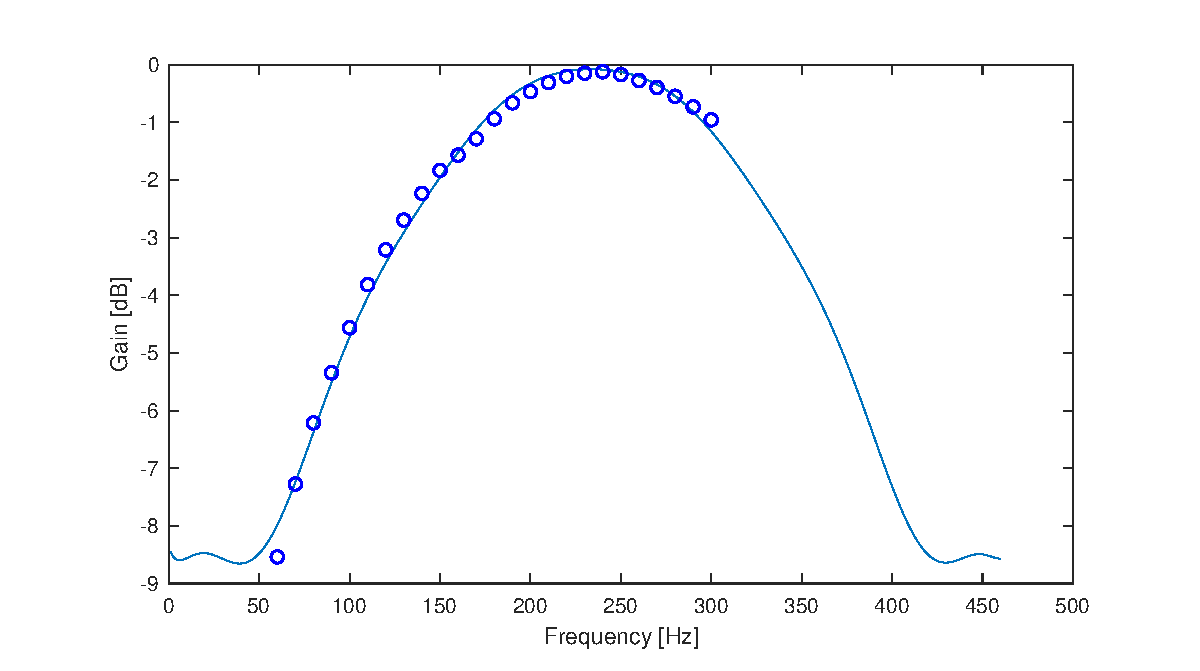
\includegraphics[width=1\textwidth]{band_pass_filter.eps}
	\caption{Inverted and zeroed estimated function (blue solid line) and inverted given data points (dots).}
		\label{fig:band_pass_filter}
\end{figure}

In \autoref{fig:band_pass_filter} it can be seen, that the \SI{-3}{\decibel} bandwidth is \SI{293}{\hertz} and that there is a gain difference of \SI{8.5}{\decibel} between the lowest given data point and the highest given data point. The bandpass filter has a center frequency of \SI{234}{\hertz}. The initial filter parameters are:

\begin{itemize}
\item Gain: $G = \SI{8.5}{\decibel}$
\item Bandwidth: $BW = 2\pi \SI{293}{\hertz} = 1841$
\item Center frequency: $\omega_0 = 2\pi \SI{234}{\hertz} = \SI{1470.3}{\second ^{-1}}$
\item Filter quality: $Q = \frac{1470.3}{1841} = 0.7986$
\end{itemize}

The transfer function corresponding to the block diagram in \autoref{fig:bandstop_filter_blockdiagram_gain} is calculated according to \autoref{eq:bandstop_filter_eq}.

\begin{equation}\label{eq:bandstop_filter_eq}
H_{stop}(s) = \text{In_Gain} \cdot \frac{s^2+\frac{\omega_0}{Q}s+\omega_0^2}{s^2+\frac{\omega_0}{Q}s(G')+\omega_0^2}
\end{equation}

    \startexplain
        \explain{$G = 1 + G'$, where $G'$ corresponds to the $\text{Gain}$ in block diagram \autoref{fig:bandstop_filter_blockdiagram_gain} and $G$ correspond to the bandpass gain}{1}
    \stopexplain


A magnitude plot resulting \autoref{eq:bandstop_filter_eq} with the formerly mentioned parameters, where the $\text{In_Gain}$ is set to \SI{0}{\decibel}, is shown in \autoref{fig:bandstop_filter_eq_bodeplot}



\begin{figure}[H]
	\centering
	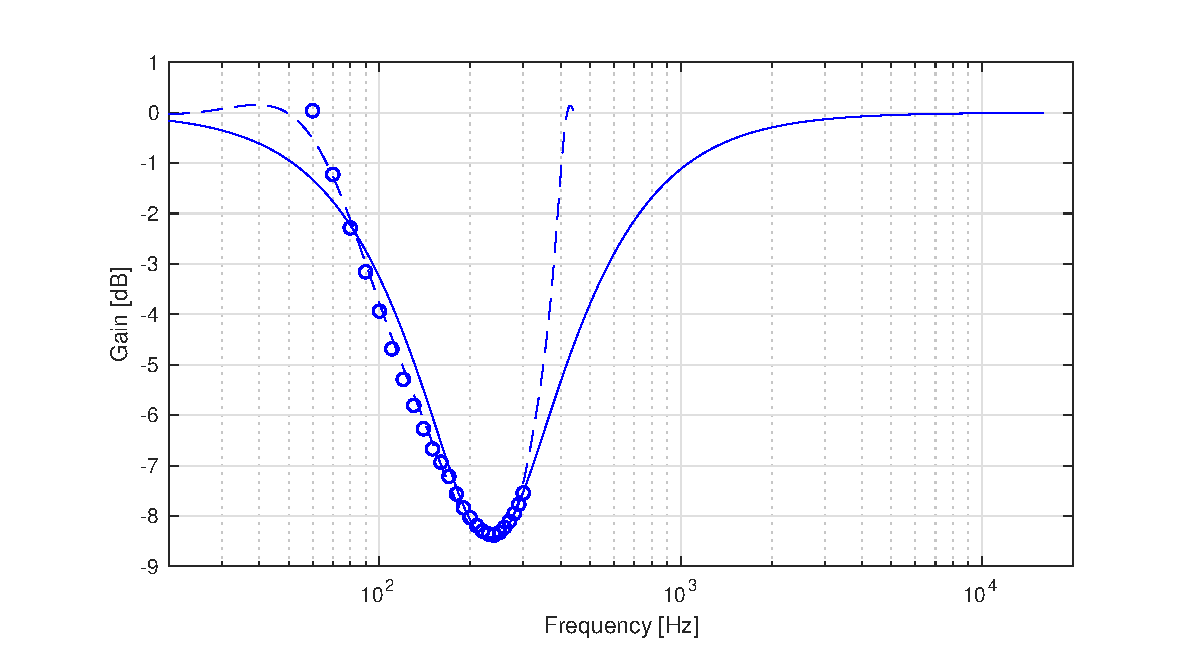
\includegraphics[width=1\textwidth]{bandstop_filter_eq_bodeplot.eps}
	\caption{Magnitude plot resulting from \autoref{eq:bandstop_filter_eq} (solid blue line) and given data points.}
		\label{fig:bandstop_filter_eq_bodeplot}
\end{figure}

On graph in \autoref{fig:bandstop_filter_eq_bodeplot} fits well to the given data points from \SI{100}{\hertz} and upwards, but at frequency below \SI{100}{\hertz} there is significant deviation. To solve this problem, the data point can be shifted to fit onto the steep slope of the filter. The disadvantage of shifting the data points to the steeper slope of the transfer function is, that the gain of the filter has to be higher. A higher filter gain has to be compensated with a higher $\text{In_Gain}$, which leads to the frequencies below \SI{60}{\hertz} and above \SI{300}{\hertz} being amplified. The data points are shifted by \SI{4}{\decibel} and the bandpass filter gain $G$ is increased by \SI{4}{\decibel}. The following \autoref{fig:bandstop_filter_eq_bodeplot_attenuated} shows the result.

\begin{figure}[H]
	\centering
	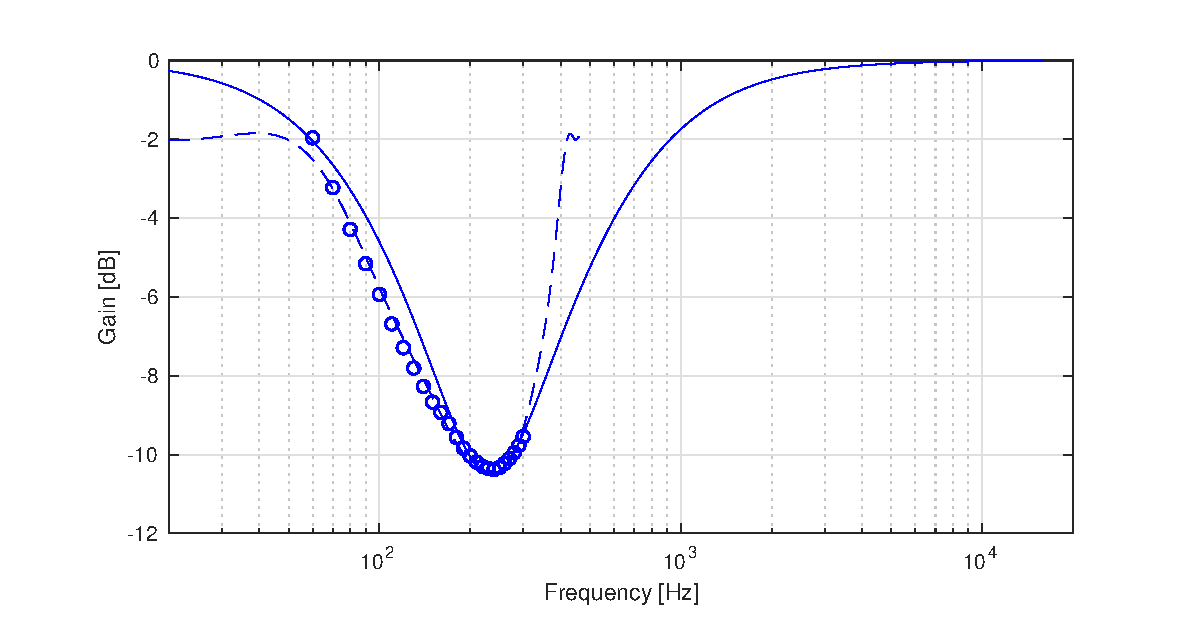
\includegraphics[width=1\textwidth]{bandstop_filter_eq_bodeplot_attenuated.eps}
	\caption{Mgnitude plot with shifted parameters (blue line) the according to\autoref{eq:bandstop_filter_eq} and shifted given data points (dots).}
		\label{fig:bandstop_filter_eq_bodeplot_attenuated}
\end{figure}


As it can be seen on \autoref{fig:bandstop_filter_eq_bodeplot_attenuated}, shifting the data points has positively affected the fit. The filter gain is therefore changed to  $G = \SI{12.5}{\decibel}$ in the parameters. Recalling from \autoref{fig:bandstop_filter_eq_bodeplot_attenuated} the filter is attenuated with \SI{4}{\decibel} and therefore the overall gain, which is denoted as $\text{In_Gain}$ shall be increased by \SI{4}{\decibel} plus the \SI{6.4}{\decibel}, which corresponds to the inverting in \autoref{fig:band_pass_filter}. According to this, the overall gain has to be \SI{10.4}{\decibel}. The final filter parameter are as follows:

\begin{itemize}
\item Gain $\text{In_Gain} = \SI{10.5}{\decibel}$
\item Gain $G = \SI{12.5}{\decibel}$
\item Bandwidth is $BW = 2\pi \SI{293}{\hertz} = 1841$
\item Center frequency is $\omega_0 = 2\pi \SI{234}{\hertz} = \SI{1470.3}{\second ^{-1}}$
\item The filter quality $Q = \frac{1470.3}{1841} = 0.7986$
\end{itemize}

The magnitude response to the formerly mentioned parameters according to \autoref{eq:bandstop_filter_eq} is illustrated in \autoref{fig:cost_filter_final}.

\begin{figure}[H]
	\centering
	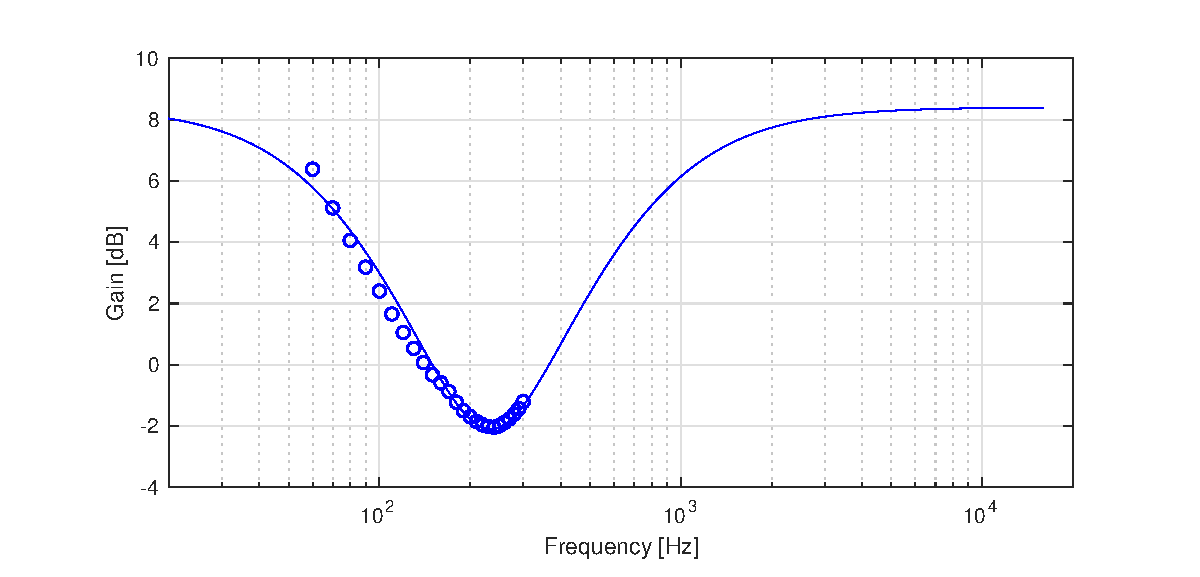
\includegraphics[width=1\textwidth]{cost_filter_final.eps}
	\caption{Magnitude plot resulting from the final parameters according to \autoref{fig:cost_filter_final}}
		\label{fig:cost_filter_final}
\end{figure}

\autoref{fig:cost_filter_final} shows, that the frequencies, that are out of the range of interest, are amplified by up to \SI{10.4}{\decibel}. This issue will later be solved with a generic bandpass filter, with a passband greater than from \SI{60}{\hertz} to \SI{300}{\hertz}.
 


\subsection{Converting the Cost Filter to Differential Equations}
In order to implement the cost filter in MATLAB and to finally generate the output signals for the loudspeaker array, the analogue designed filter has to be converted into a digital filter. The conversion will be excecuted by using the bilinear transformation without pre-wrapping, which converts analogue filters intro \gls{iir} filters. The reason to neglect the use of pre-wrapping in this context, is that the filter is designed to act upon low frequency with compared to the Nyquist rate. When the filter is designed to act upon low frequencies with respect to the Nyquist rate, the pre-wrapping only has little effect on the crossover position compared to a filter that is acting upon frequencies close to the Nyquist rate. With the transformation a transition is made from the continous Laplace domain in \autoref{eq:bandstop_filter_eq} into discrete Laplace domain. The bilinear transformation is excecuted as follows:

\begin{equation}\label{eq:bandstop_filter_bilinear}
H_{stop}(z) = H_{stop}(s) \mid_{s=\frac{2}{T_s}\frac{z-1}{z+1}} 
\end{equation}

    \startexplain
        \explain{$H(z)$ is the digital transfer function}{1}
        \explain{$T_s$ is the sample time}{\si{\second}}
    \stopexplain

Applying the transformation \autoref{eq:bandstop_filter_bilinear} to the analogue cost filter equation results in \autoref{eq:bandstop_filter_eq_z}.

\begin{equation}\label{eq:bandstop_filter_eq_z}
H_{stop}(s) = \text{In_Gain} \cdot \frac{(\frac{2}{T_s}\frac{z-1}{z+1})^2+\frac{\omega_0}{Q}\frac{2}{T_s}\frac{z-1}{z+1}+\omega_0^2}{(\frac{2}{T_s}\frac{z-1}{z+1})^2+\frac{\omega_0}{Q}\frac{2}{T_s}\frac{z-1}{z+1}(G)+\omega_0^2}
\end{equation}

\autoref{eq:bandstop_filter_eq_z} is changed such that the parameters simplified to a- and b-coefficients. The following \autoref{eq:bandstop_filter_peak_att} describes the digital transfer function.


\begin{equation}\label{eq:bandstop_filter_peak_att}
        H_{stop}(z) =  \text{In_Gain} \cdot \frac{z^2 \cdot a_{stop1} + z \cdot a_{stop2} + a_{stop3}}{z^2 \cdot b_{stop1} + z \cdot b_{stop2} + b_{stop3}}
    \end{equation}
    
    \startexplain
     \explain{$H_{stop}(z)$ is the digital transfer function for the stop filter}{\si{1}}
     \explain{$b_{stop1} = 4 \cdot Q + \omega_0 \cdot G \cdot T_s \cdot 2 + \omega_0^2 \cdot T_s^2 \cdot Q  $ }{\si{1}}
     \explain{$b_{stop2} =-8 \cdot Q + 2 \cdot  \omega_0^2 \cdot T_s^2 \cdot Q$ }{\si{1}}
     \explain{$b_{stop3} = 4 \cdot Q - 2 \cdot \omega_0 \cdot T_s \cdot G + \omega_0^2 \cdot T_s^2 \cdot Q$ }{\si{1}}
     \explain{$a_{stop1} = 4 \cdot Q + 2 \cdot \omega_0 \cdot T_s + \omega_0^2 \cdot T_s^2 \cdot Q$ }{\si{1}}
     \explain{$a_{stop2} = -8 \cdot Q + 2 \cdot  \omega_0^2 \cdot T_s^2 \cdot Q$ }{\si{1}}
     \explain{$a_{stop3} = 4 \cdot Q - 2 \cdot \omega_0 \cdot T_s + \omega_0^2 \cdot T_s^2 \cdot Q$ }{\si{1}}
    \stopexplain

The last step is to convert the cost filter from the discrete Laplace domain into a differential equation in the discrete time domain. The following steps in \autoref{eq:z_to_n} contain the domain transformation.



\begin{subequations}\label{eq:bandstop_filter_peak_n}
\begin{alignat}{2}
 H_{stop}(z)=\frac{Y(z)}{X(z)} &=  \text{In_Gain} \cdot \frac{z^2 \cdot a_{stop1} + z \cdot a_{stop2} + a_{stop3}}{z^2 \cdot b_{stop1} + z \cdot b_{stop2} + b_{stop3}} \label{eq:bandstop_filter_peak_n_1}\\
 \Downarrow\\
 H_{stop}(z)=\frac{Y(z)}{X(z)} &=  \text{In_Gain} \cdot \frac{a_{stop1} + z^{-1} \cdot a_{stop2} +  z^{-2} \cdot a_{stop3}}{b_{stop1} + z^{-1} \cdot b_{stop2} +  z^{-2} \cdot b_{stop3}}  \label{eq:bandstop_filter_peak_n_2}
\end{alignat}
\end{subequations}


\begin{subequations}\label{eq:z_to_n}
    \centering
$\Updownarrow$
\begin{multline}\label{eq:z_to_n3}
        Y(z) \cdot (b_{stop1} + b_{stop2} \cdot z^{-1} + b_{stop3} \cdot z^{-2}) \\ = X(z) \cdot \text{In_Gain} \cdot (a_{stop1} + a_{stop2} \cdot z^{-1} + a_{stop3} \cdot z^{-2})
\end{multline}
       \centering
$\Updownarrow$
\begin{multline}\label{eq:z_to_n4}
         Y(z) \cdot b_{stop} + Y(z) \cdot b_{stop2} \cdot z^{-1} + Y(z) \cdot b_{stop3} \cdot z^{-2} \\=  \text{In_Gain} \cdot (X(z) \cdot a_{stop1} + X(z) \cdot a_{stop2} \cdot z^{-1} + X(z) \cdot  a_{stop3} \cdot z^{-2})
    \end{multline}
    \centering
    $\Downarrow Z^{-1}$
\begin{multline}\label{eq:z_to_n5}
         b_{stop1} \cdot y[n] + b_{stop2} \cdot y[n-1] + b_{stop3} \cdot y[n-2] \\=  \text{In_Gain} \cdot (a_{stop1} \cdot x[n] +  a_{stop2} \cdot x[n-1] + a_{stop3} \cdot x[n-2])
    \end{multline}
    \centering
    $\Updownarrow$
\begin{multline}\label{eq:z_to_n6}
         b_{stop1} \cdot y[n] =  \text{In_Gain} \cdot (a_{stop1} \cdot x[n] + a_{stop2} \cdot x[n-1] + a_{stop3} \cdot x[n-2]) \\-  b_{stop2} \cdot y[n-1] - b_{stop3} \cdot y[n-2]
    \end{multline}
    \centering
    $\Updownarrow$
\begin{multline}\label{eq:z_to_n7}
         y[n] = \frac{\text{In_Gain}  \cdot a_{stop1}}{b_{stop1}} \cdot x[n] + \frac{\text{In_Gain}  \cdot a_{stop2}}{b_{stop1}} \cdot x[n-1] \\+  \frac{\text{In_Gain}  \cdot a_{stop3}}{b_{stop1}} \cdot x[n-2] -  \frac{b_{stop2}}{b_{stop1}} \cdot y[n-1] - \frac{b_{stop3}}{b_{stop1}} \cdot y[n-2]
    \end{multline}
    
    \startexplain
     \explain{$y[n]$ is the output sample.}{\si{1}}
     \explain{$x[n]$ is the input sample.}{\si{1}}
    \stopexplain
 \end{subequations}


\section{The Beamforming filter}
The beamforming filter is not as easy to design as the cost filter, since there are exact requirements on phase and the gain characteristics for the beamforming to work. Therefore the phase have to be taken into account when deciding on a filter type. From the data point from the \ref{sec:opt_result} it can be seen, that the phase requirments are close to linear in the frequency range of interest. Therefore the filter will be a linear phase \gls{fir} filter. The advantage of choosing a \gls{fir} filter is, that the impulse response of the filter just has to be symmetric in order to result in a linear phase response. This means, that it is only necessary to optimize one half of the impulse response. It can then be augmented with a mirrored version of it self. This method will result in a linear phase. One disadvantage in this particular case is, that the filter has to act upon frequencies that are small compared to the sample frequency. This means, that the resulting filter will have many taps. \\

A modified version of the genetic optimization algorithm from \autoref{sec:genetic_implememtation} will be used to find an optimized impulse response of the filter. \autoref{ax:opt_imp_filter} explains the modifications that have been undertaken. To optimize the impulse response of the filter, an initial estimate of the impulse respond has to be determined. First, the given data is regressed and extrapolated by the use of the \texttt{polyfit()} and \texttt{polyval()} functions in MATLAB. For the gain requirements, a second order regression is done, for the phase, a linear regression is done. The reason to extrapolate with only an order of two on the regressed gain, is to keep the number of taps small and ensure that there is a good fit at the outer boundaries of frequency range of interest. By doing an extrapolation, the transfer function outside of the frequency range of interest still has to follow the second order polynomial and does not take on some steep shape. Another benefit might be, that at the of the boundary of the frequency range of interest, there is no abrupt end of the fitness evaluation, which might make the genetic algorithm converge better. It has to be noted, that it is not expected, that at frequencies outside the frequency range from \SI{60}{\hertz} to \SI{300}{\hertz} beamforming will occur because of the extrapolation. The used way to estimate the impulse response is to transform all of data points, that are given as polar coordinates, into a complex rectangular transfer function and calculate the real values of the \gls{ifft}. The polar to rectangular transform is done as described in \autoref{eq:pol_to_regt}

\begin{equation}\label{eq:pol_to_regt}
x=r \cos(\phi)+j \cdot r \sin(\phi)
\end{equation}


    \startexplain
    	\explain{$\phi$ is the angle of the transfer function}{\si{radian}}
        \explain{$r$ is the amplitude of the transfer function}{\si{1}}
        \explain{$j$ is the imaginary unit}{\si{1}}
    \stopexplain

The real of the \gls{ifft} gives an estimated impulse response but with a scaled cross over point, meaning that the cross over point follows the scaling of the sample frequency. With a sample rate of \SI{44.1}{\kilo\hertz}. The following  \autoref{fig:ir_estimate_non_scaled} shows the transfer function of the estimated impulse response. 

\begin{figure}[H]
	\centering
	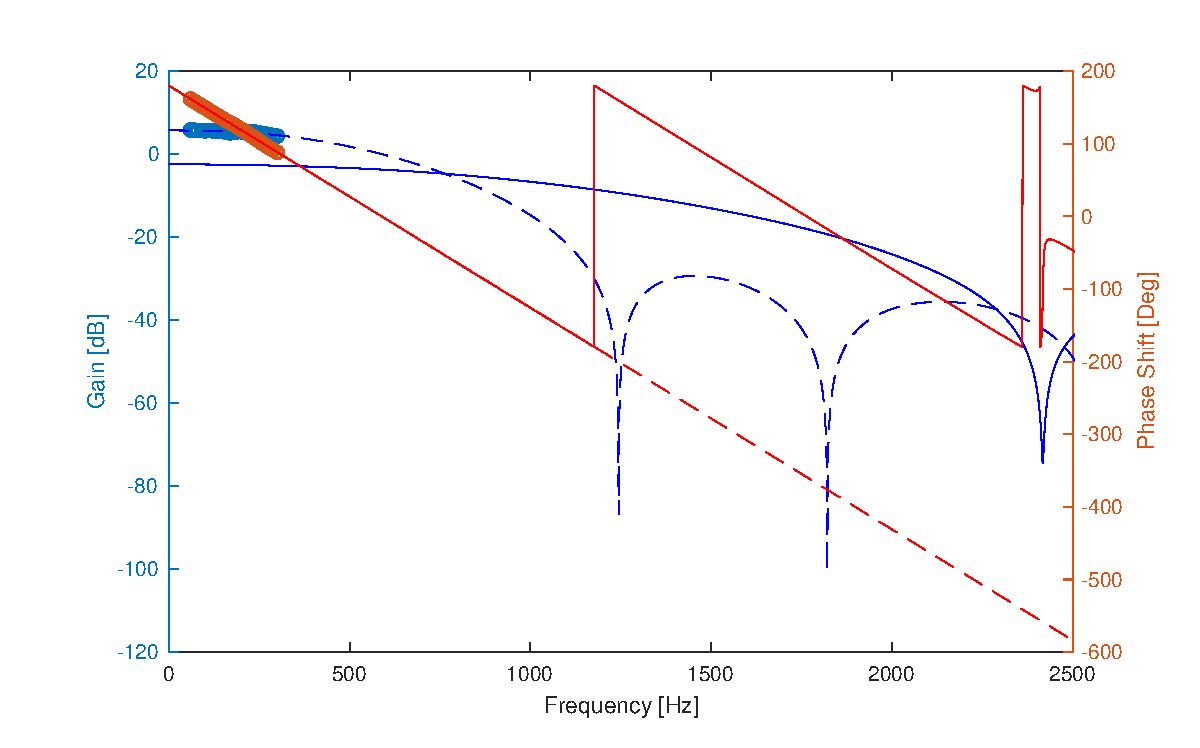
\includegraphics[width=1\textwidth]{ir_estimate_non_scaled.eps}
	\caption{Transfer function resulting from the estimated impulse response and regressed transfer function. The dashed lines show the regressed transfer function, that is needed for the beamforming filter,  where the blue dashed line is the gain and the red dashed line is the phase. The frequency range of interest is between \SI{60}{\hertz} to \SI{300}{\hertz}. The solid lines denotes the transfer function of the estimated impulse response, where the blue solid line is the gain and the red solid line is the phase. The circles denote the filter requirement datapoints from the optimization result.}
		\label{fig:ir_estimate_non_scaled}
\end{figure}


It can be seen, that the cutoff frequency is too high and that the gain at the frequency of interest is too low. 
%The impulse response corresponding to the estimated transfer function in \autoref{fig:ir_estimate_non_scaled} is shown in \autoref{fig:ir_estimate_mirror}. The impulse response had to be circle shifted from the initial calculation to account for a phase offset, that was in the result from the \gls{ifft}. 
For the optimization it is only one half of the impulse response, that needs to be optimized, because the phase is required to be linear. The following \autoref{fig:ir_estimate_non_mirror} shows the half impulse response for the optimization.

\begin{figure}[H]
	\centering
	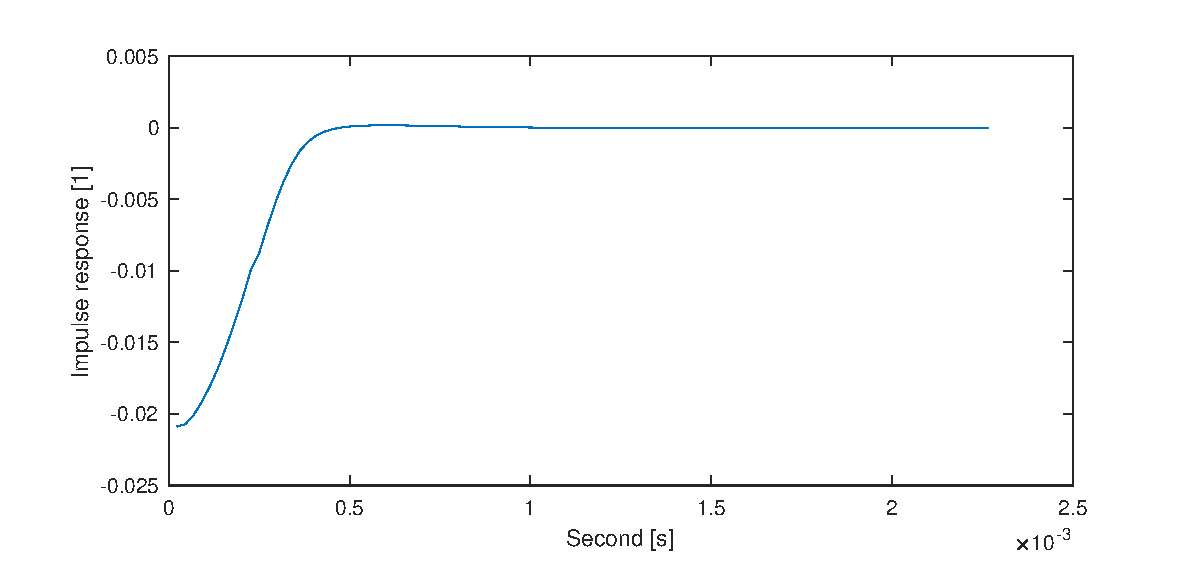
\includegraphics[width=1\textwidth]{ir_estimate_non_mirror.eps}
	\caption{Impulse response for optimization initialization, without the mirrored version attached.}
		\label{fig:ir_estimate_non_mirror}
\end{figure}

To later use the impulse response, that results from the optimization, the mirrored version of the impulse response is added to the left side of the graph. To tweak the phase such that it fits the desired phase, the impulse response is circle shifted until the phase fits. The following \autoref{fig:ir_estimate_mirror} shows the result and the impulse response for the solid line in \autoref{fig:ir_estimate_non_scaled} by changing the phase manually.



\begin{figure}[H]
	\centering
	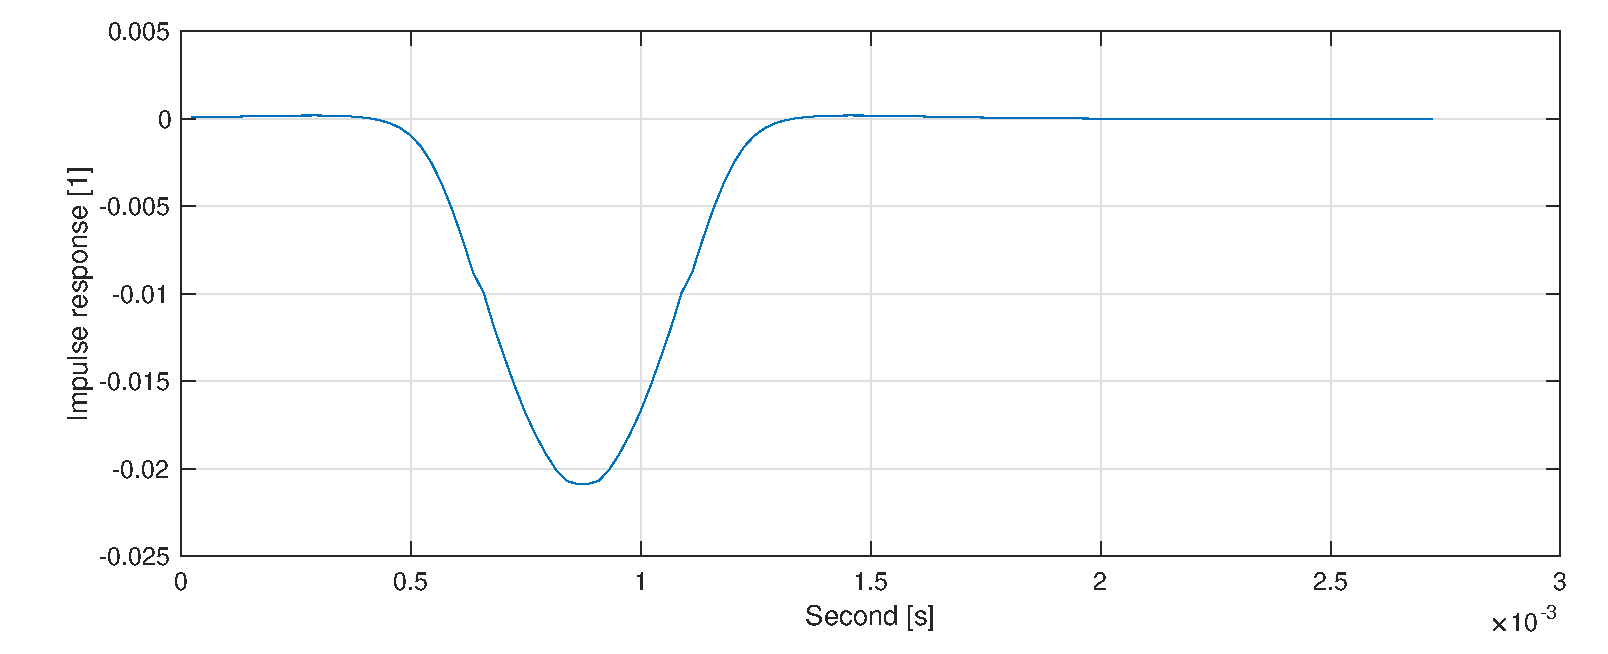
\includegraphics[width=1\textwidth]{ir_estimate_mirror.eps}
	\caption{Impulse response with the mirrored version attached, circle shifted to fit phase requirements.}
		\label{fig:ir_estimate_mirror}
\end{figure}


It can be seen in \autoref{fig:ir_estimate_non_mirror}, that the impulse response has to be modified in order to make a good estimate. The way to decrease the cutoff frequency is to extend the part of the impulse respond that has the highest amplitude, which also make the impulse response longer. %Thinking about the theory of the \gls{fir} filter, that the lower cross over, the higher order the filter have to be and therefore the impulse respond gets longer.  
The following  \autoref{fig:ir_estimate_scaled} shows the transfer function of the impulse response which is extended as described and shown in \autoref{fig:ir_estimate_mirror_scale}.


\begin{figure}[H]
	\centering
	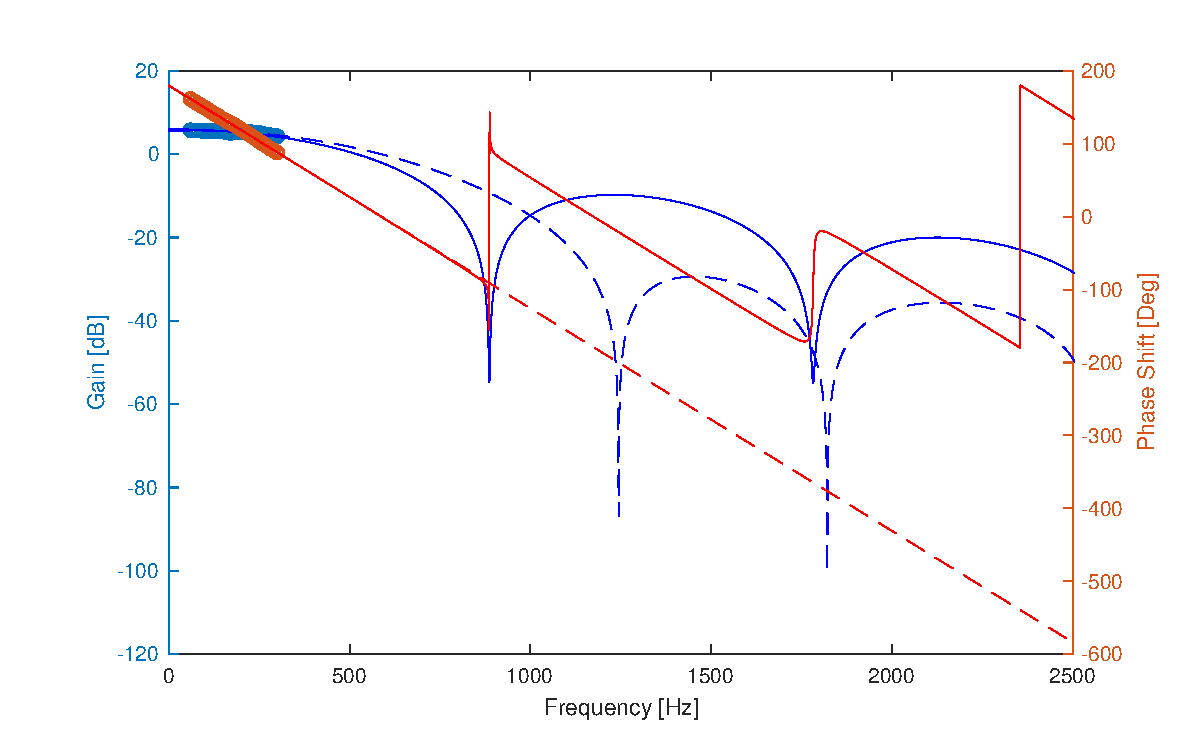
\includegraphics[width=1\textwidth]{ir_estimate_scaled.eps}
	\caption{Transfer function of the estimated impulse response after extending it. The dashed lines show the regressed transfer function, that is needed for the beamforming filter,  where the blue dashed line is the gain and the red dashed line is the phase. The solid lines denotes the transfer function of the extended estimated impulse response, where the blue solid line is the gain and the red solid line is the phase. The circles denote the filter requirement datapoints from the optimization result.}
		\label{fig:ir_estimate_scaled}
\end{figure}


It can be seen on \autoref{fig:ir_estimate_scaled} that the elongation of the impulse response has the desired effect. The initial impulse response that will be used for the optimization is the elongated impulse response, where the first half of the impulse is removed as described above. The following  \autoref{fig:ir_estimate_mirror_scale} shows the impulse response that corresponds to the transfer function in \autoref{fig:ir_estimate_scaled}

\begin{figure}[H]
	\centering
	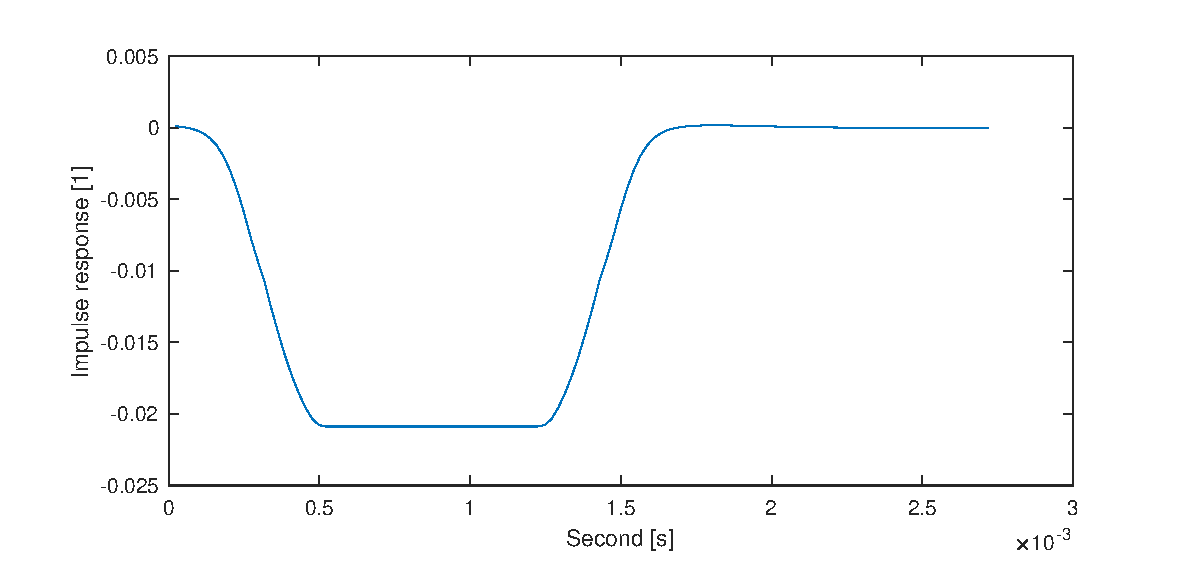
\includegraphics[width=1\textwidth]{ir_estimate_mirror_scale.eps}
	\caption{Elongated initial impulse response estimate.}
		\label{fig:ir_estimate_mirror_scale}
\end{figure}


%The fit on \autoref{fig:ir_estimate_scaled} seems to fit well, but to determined a visual fitness \autoref{fig:ir_estimate_scaled_close} shows a closer look on the frequency of interest.


\begin{figure}[H]
	\centering
	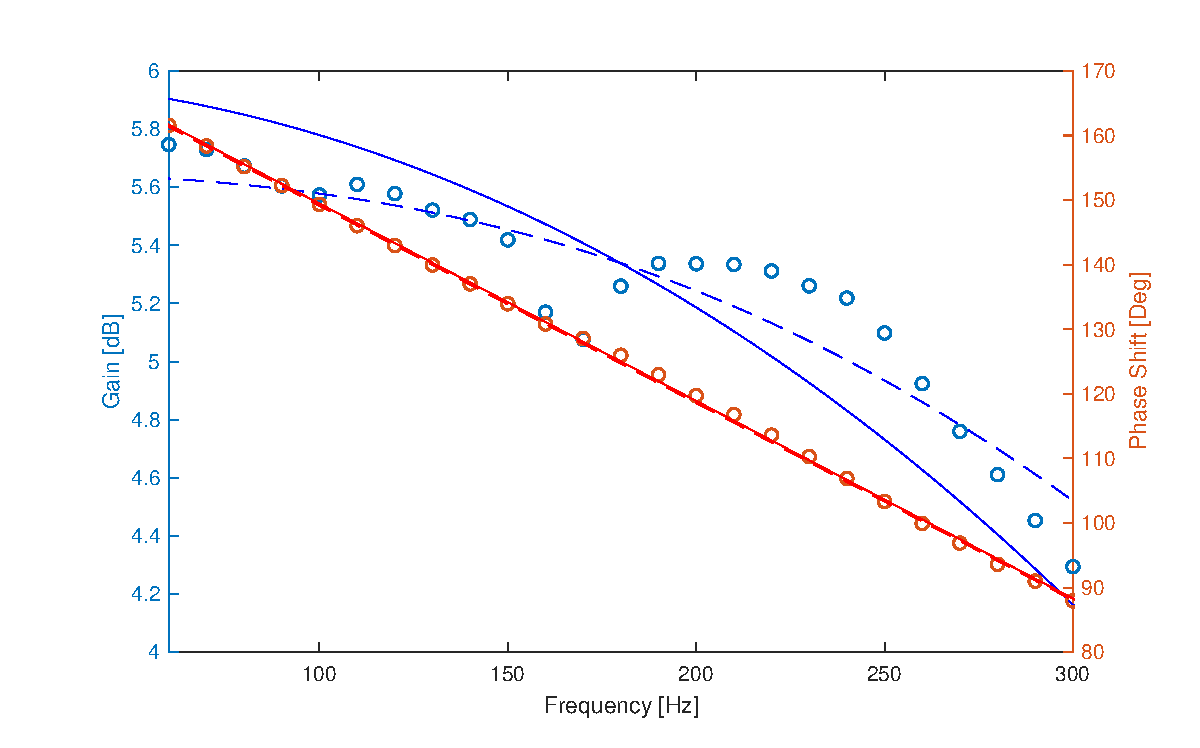
\includegraphics[width=1\textwidth]{ir_estimate_scaled_close.eps}
	\caption{Transfer function of the elongated estimated impulse response in the frequency range of interest. The dashed lines show the regressed transfer function, that is needed for the beamforming filter,  where the blue dashed line is the gain and the red dashed line is the phase. The solid lines denotes the transfer function of the extended estimated impulse response, where the blue solid line is the gain and the red solid line is the phase. The circles denote the filter requirement datapoints from the optimization result.}
		\label{fig:ir_estimate_scaled_close}
\end{figure}

\autoref{fig:ir_estimate_scaled_close} is a zoomed in version of \autoref{fig:ir_estimate_scaled}.
As it can be seen at \autoref{fig:ir_estimate_scaled}, the cut off is lowered and the gain is automatically raised to the wanted area. The closer look on frequency area of interest, provided in \autoref{fig:ir_estimate_scaled_close}, shows that the fit is close, but the gain can be optimized. Recalling from earlier, a linear phase \gls{fir} filter has to have symmetrical impulse response and therefore the impulse response, where the mirrored version is not added will be used as initial guess for a \gls{ga}. To optimize the impulse response there will be used high probabilities for mutation and crossover. The reason to use high probability for mutation, is that the shape of the impulse response is changed a bit for every mutation, and it is the shape, that needs to be changed to result in optimal \gls{fir} filter coefficients. In the mutation part, the following mutations are done.

\begin{itemize}
\item One single random chosen point in the impulse response is change by increasing or decreasing its value.
\item One random chosen area of the impulse response is changed by moving it up and down wards with the shape of a Gaussian bell curve, where $\mu$ and $\sigma$ are chosen randomly.
\item An up-sampling is done on the impulse response with a factor of ten. After the up-sampling, the value at time zero is copied and used as the new zero point after the impulse response is shifted one sample to the right. The reason to up-sample is the shifting can therefore be applied with a finer resolution. This technique leads to a closer fit than it is possible to achieve without upsampling. The up-sampling is done with linear interpolation. This mutation ends with down sampling with a factor of ten such that the impulse respond is at the same length as at the beginning.
\item The impulse response is multiplied with a randomly chosen factor. 
\end{itemize}

After applying the mutation, the last point of the impulse response is used as the \gls{dc} offset and the offset will be subtracted from the impulse response, such that the impulse response ends with an amplitude of zero. 

\section{Result}
The genetic algorithm did converge towards the regressed transfer function. The following \autoref{fig:filter_coefficient} shows the optimized impulse response.

 \begin{figure}[H]
	\centering
	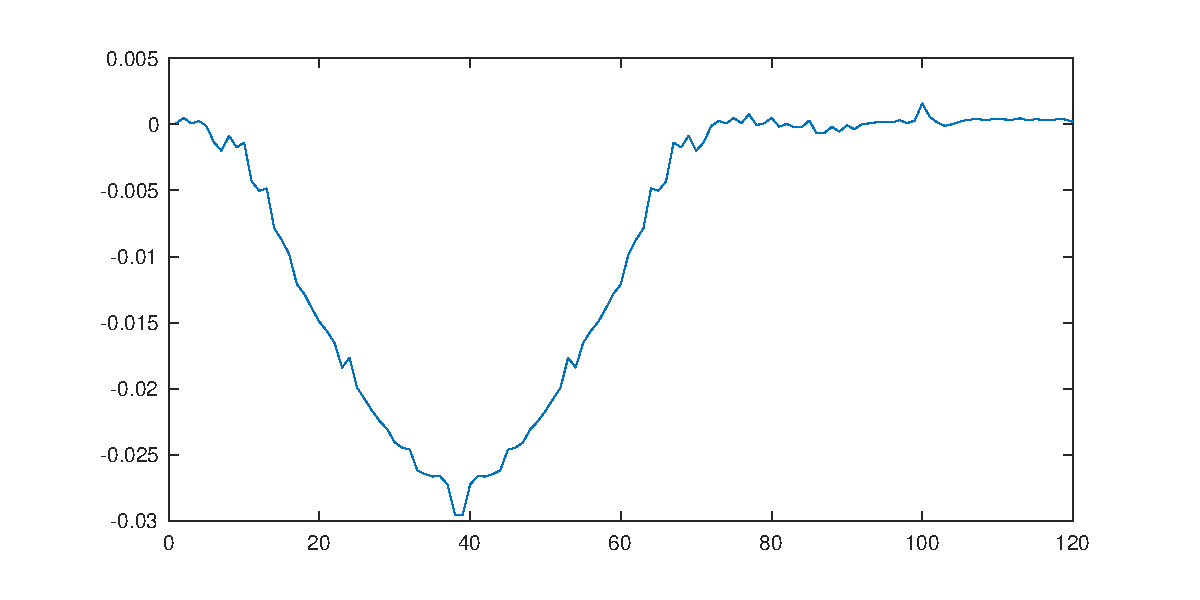
\includegraphics[width=1\textwidth]{filter_coefficient.eps}
	\caption{Optimized impulse response.}
		\label{fig:filter_coefficient}
\end{figure}

The transfer function corresponding to the optimal impulse response shown in\autoref{fig:filter_coefficient} is illlustrated \autoref{fig:filter_vs_reg}.

\begin{figure}[H]
	\centering
	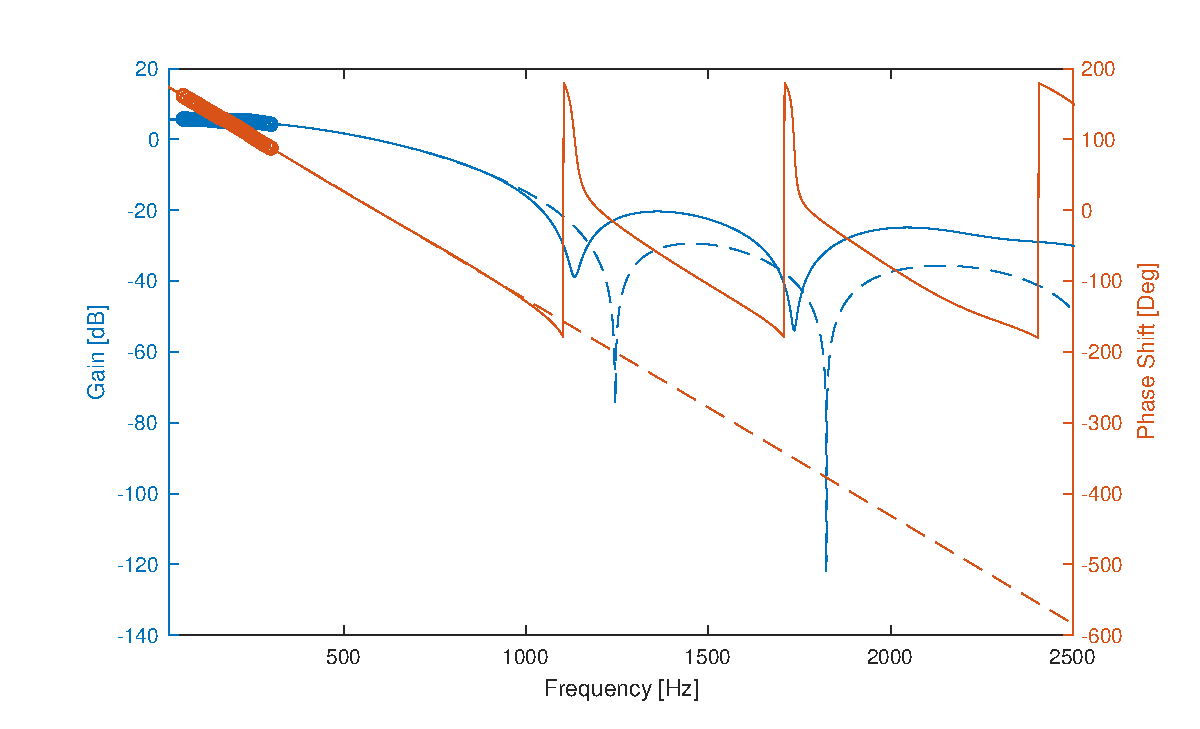
\includegraphics[width=1\textwidth]{filter_vs_reg.eps}
	\caption{Transfer function corresponding to the optimal impulse response. The dashed lines show the regressed transfer function, that is needed for the beamforming filter,  where the blue dashed line is the gain and the red dashed line is the phase. The solid lines denotes the transfer function of the extended estimated impulse response, where the blue solid line is the gain and the red solid line is the phase. The circles denote the filter requirement datapoints from the optimization result.}
		\label{fig:filter_vs_reg}
\end{figure}


\autoref{fig:filter_vs_reg} shows, that the optimized transfer function fits the regressed filter op to \SI{1}{\kilo\hertz}. The weighting function in the genetic algorithm was only taking frequencies up to \SI{1}{\kilo\hertz} into account for the fitness value. Therefore, higher frequencies do not fit. This does not have any disadvantages regarding the use of the filter. Since the phase can be changed only by circle shifting the impulse response, the phase only was assigned half of weight compared to the gain, when calculating the fitness values during the optimization. A closer look on the the frequency range of interest is given in \autoref{fig:filter_vs_data_finish}. In \autoref{fig:opt_res_finish}, also transfer function of the cost filter and polar plots of the expected directional characteristics of the array with optimal parameters and the parameters resulting from the beamforming filter based on the unaugmented analytical model are shown.


\begin{figure}[H]
\begin{subfigure}[c]{0.5\textwidth}
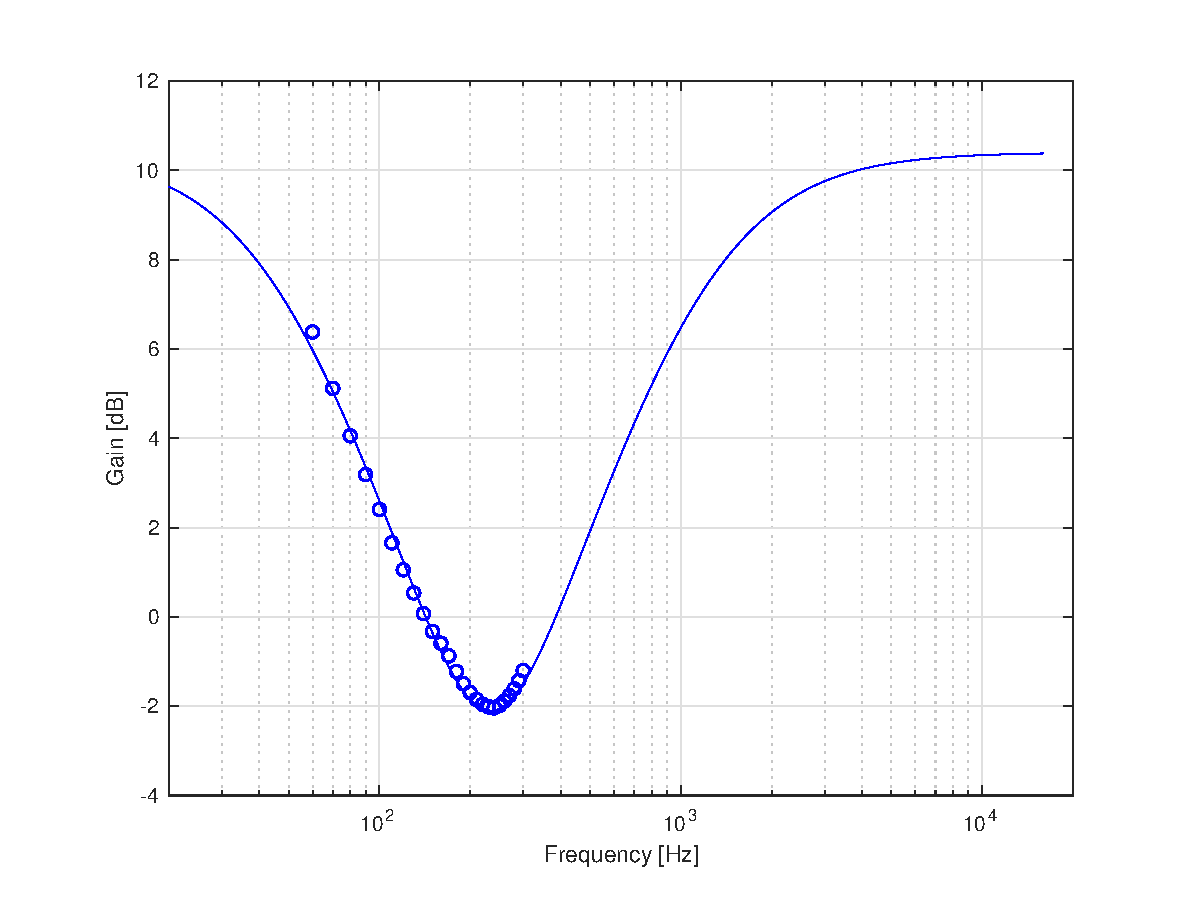
\includegraphics[width=0.85\textwidth]{opt_c_final.eps}
\subcaption{Amplitude response of the cost filter}
\label{fig:opt_res_a_finish}
\end{subfigure}
\begin{subfigure}[c]{0.5\textwidth}
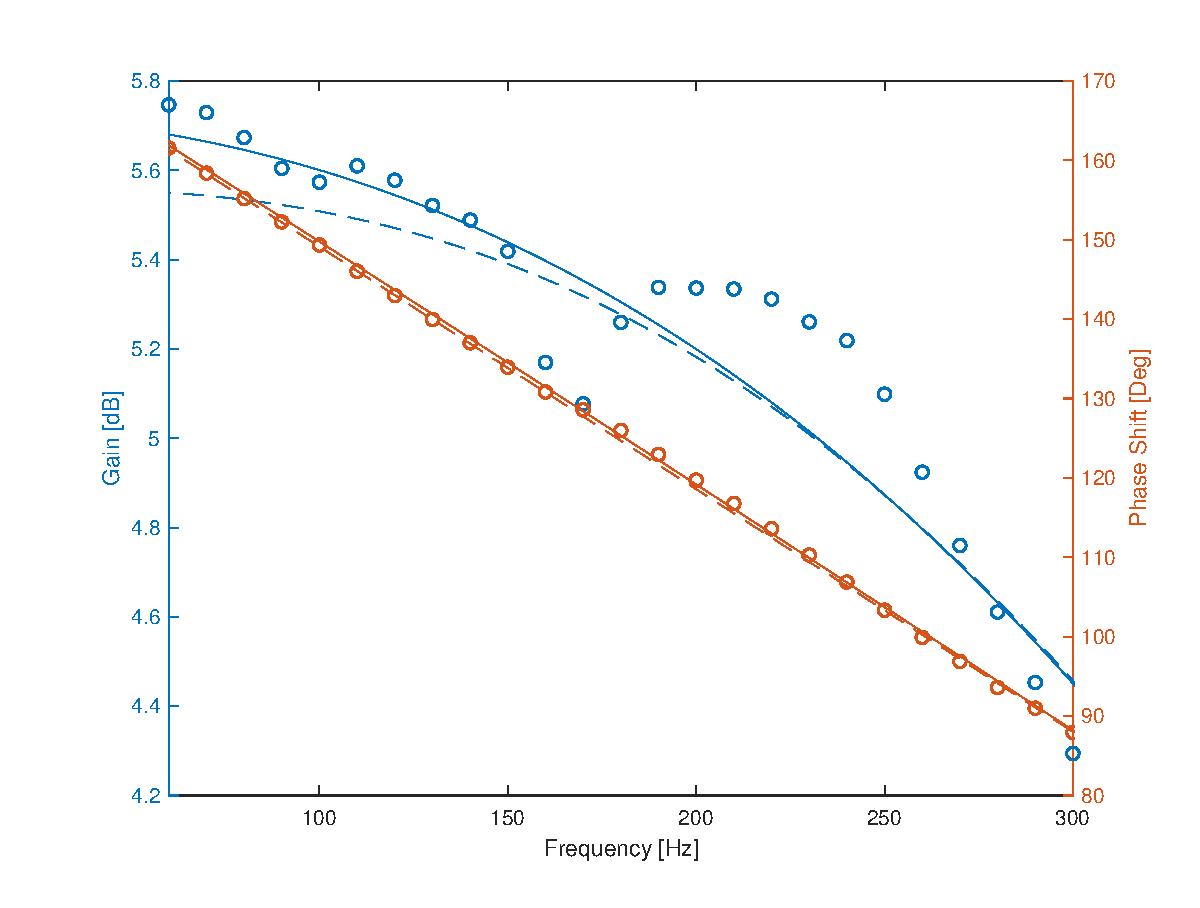
\includegraphics[width=0.95\textwidth]{filter_vs_data.eps}
\subcaption{Transfer function of the beamforming filter}
\label{fig:filter_vs_data_finish}
\end{subfigure}\\
\hspace{0.1\textheight}
\begin{subfigure}[c]{0.5\textwidth}
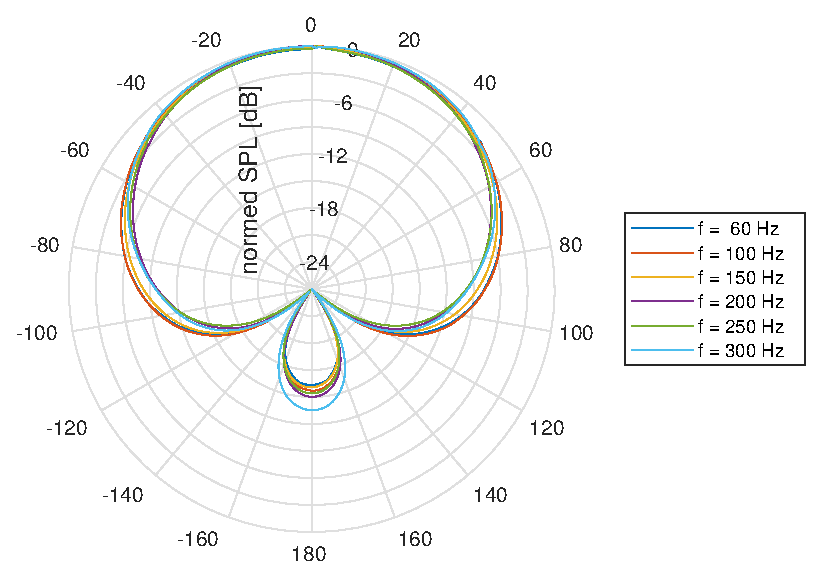
\includegraphics[width=0.95\textwidth]{opt_c.eps}
\subcaption{Expected directional characteristics, optimal}
\label{fig:opt_res_c_finish}
\end{subfigure}
\begin{subfigure}[c]{0.5\textwidth}
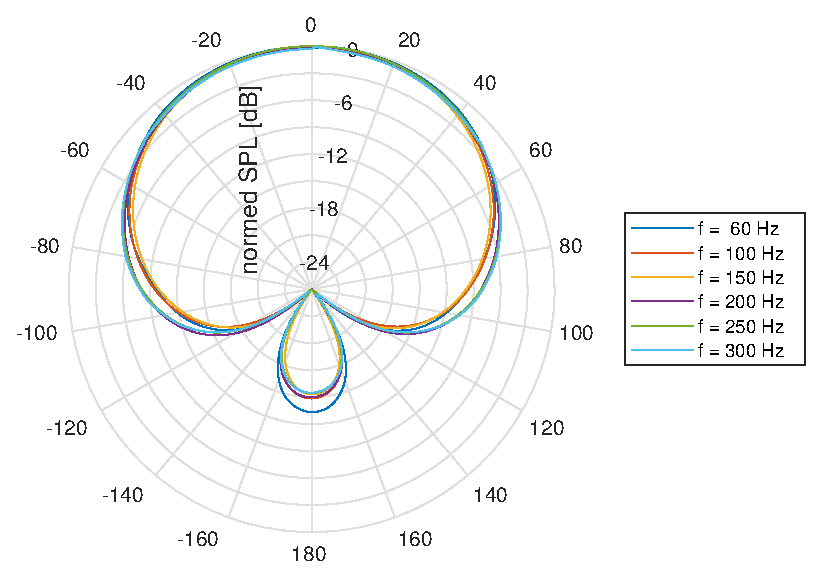
\includegraphics[width=0.95\textwidth]{polar_filtered.eps}
\subcaption{Expected directional characteristic, filtered}
\label{fig:polar_filtered_finish}
\end{subfigure}
\caption{Results of the filter design, transfer functions and expected directional characteristics for the loudspeaker array, based on unaugmented analytical model \ref{ax:directional_2}, \textcolor{green3}{\texttt{Lx}}\,$=$\,\SI{0.4}{\meter}, \textcolor{green3}{\texttt{Ly}}\,$=\,$\SI{-0.4}{\meter}}
		\label{fig:opt_res_finish}
\end{figure}


\section{Effectiveness of Cost Filtering} 
For practical reasons, the beamforming cost, to which the cost filter has been fit, has been calculated from the optimal datapoints for the beamforming filter, opposed to the filter curve that is actually used for beamforming (both visible in \autoref{fig:polar_filtered_finish}). Therefore it has to be checked, what frequency response from the array can actually be expected, taking to account, that the beamforming will be excecuted with the the beamforming filter instead of the optimal parameters. \autoref{fig:end_spl} shows the sum of the beamforming cost calculated with the beamforming filter and the cost filter that has been implemented previously. If the implemented cost filter was based on the beamforming cost corresponding to the beamforming filter, then the graph should show a linear response at a deviation of \SI{0}{\decibel}. Opposed to that, some deviation from a linear response has to be expected, due to the cost filter being fit to the cost derived from the optimal values. The deviation in the order of magnitude of \SI{\pm 1.3}{\decibel} is deemed negligible.
%It might be interesting to look at the resulting magnitude response of the beamforming array with filtered data. The \autoref{fig:end_spl} shows the magnitude plot of the analytical model where the filter parameters is  added.

\begin{figure}[H]
	\centering
	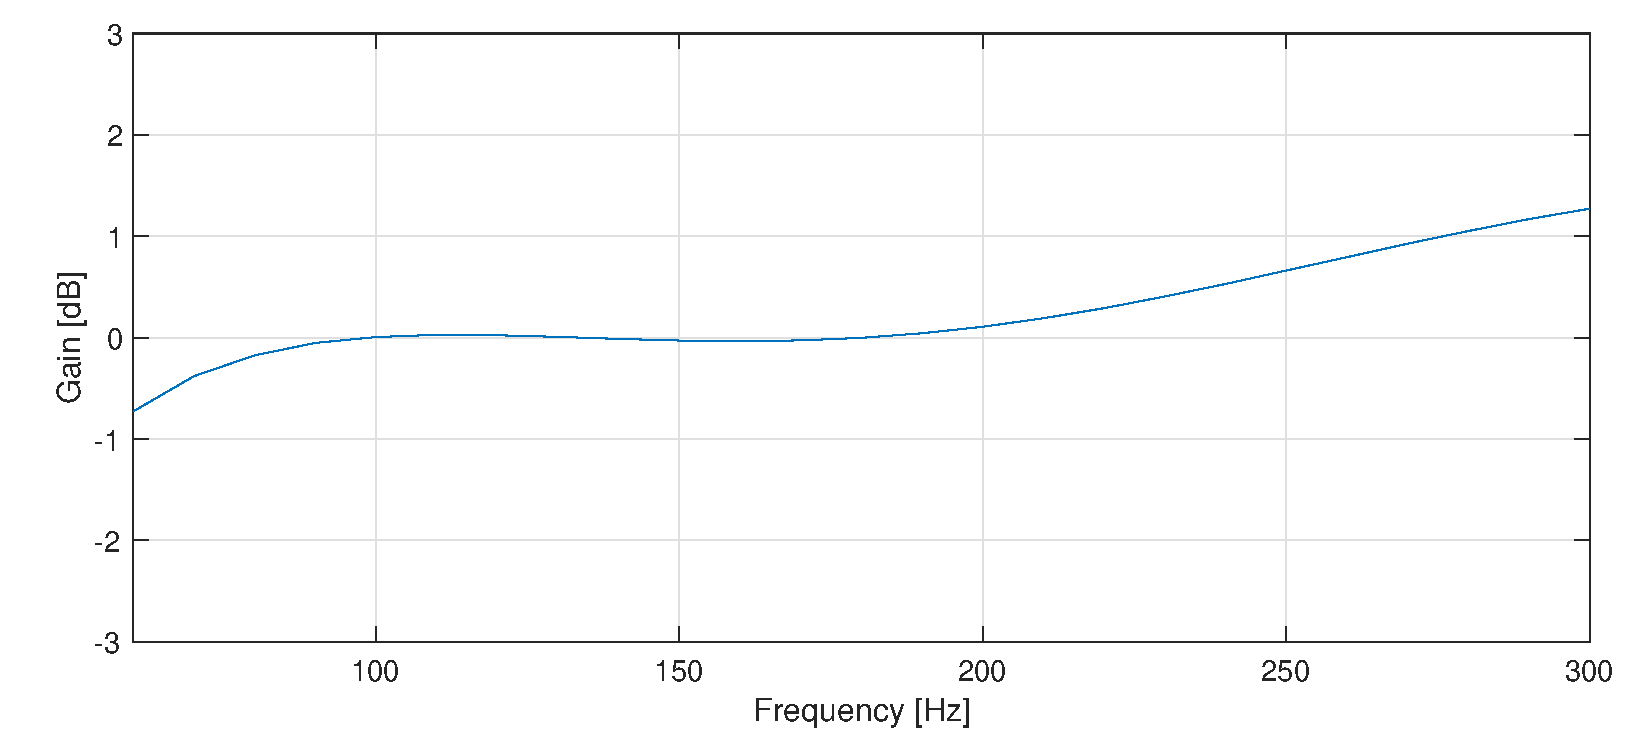
\includegraphics[width=1\textwidth]{end_spl.eps}
	\caption{Cost Deviation due to filtered beamforming parameters.}
	%The figure shows the calculated \si{\decibel} different in frequency, where the cost filter is added to the \gls{fir} filter. It has to be remembered that the cost filter is calculated from the original data and not the regressed data, and therefore the frequency response is not flat compare to if the cost filter was based on the regressed data}
		\label{fig:end_spl}
\end{figure}



\section{Conclusion of filter design}
It can be concluded that it is possible to design the cost filter as a band stop \gls{iir} filter and the beamforming filter as a low pass \gls{fir} filter. It can also be concluded that the filter does not change the expected directional characteristics of the loudspeaker array significantly, it actually only differs from the optimum directional characteristics less than or equal to \SI{1}{\decibel} for all frequencies, both in the back and in the sides of the polar plot \autoref{fig:opt_res_finish}.





